\chapter[Assessment of Parkinson's disease]{Assessment of Parkinson's disease}
\label{ch5}

\section{State of knowledge}
\label{ch5_1}

Over the last few decades, objective paraclinical methods such as the analysis of digitized hand-writing~\cite{Drotar2014, Faundez-Zanuy2014, Drotar2015, Mucha2018a}, computerized freezing of gait evaluation~\cite{Factor2014, Rocha2014}, or the acoustic analysis of dysarthric speech~\cite{Mekyska2011b_eng, Eliasova2013, Mekyska2015, Smekal2015c} have been developed. In terms of PD, the studies in which such methods have been applied have focused mainly on parkinsonian symptoms identification, description of the relationships between motor and non-motor symptoms of the disease, overall severity of PD estimation, etc. In theory, voice/speech, movement (e.\,g. gait), hand-writing and similar actions/signals can be digitized and processed remotely on computer. After that, modern signal processing techniques, statistical analyses, and/or machine learning algorithms can be used to extract a~wide range of parameters that can be integrated into a~decision support system that can eventually be used in clinical practice to enable clinicians to use such data to support their decision making when diagnosing, assessing, or monitoring the progress of PD. However, to reach this point, more studies need to be performed. 

In terms of HD in PD (i.\,e. the hypothesis is that quantification of voice/speech deficits in HD can be used to indirectly assess other non-speech symptoms of PD), especially studies that bring more insight into pathological mechanisms behind a~variety of voice/speech disorders accompanying HD and other motor and non-motor symptoms of PD are yet to be employed. If such pathological mechanisms are present and precisely described, it is likely that carefully-planned and sensitive acoustic analysis of voice/speech can be used to assess these motor and non-motor symptoms, or possibly predict their future evolution in time. 

So, with these ideas in mind, clinical rating scales that are nowadays being commonly used to quantify motor and non-motor symptoms of PD such as Unified Parkinson's Disease Rating Scale (UPDRS)~\cite{Fahn1987}, Non-Motor Symptoms Scale (NMSS)~\cite{Chaudhuri2007}, Beck Depression Inventory (BDI)~\cite{Beck2000}, Freezing Of Gait questionnaire (FOG-Q)~\cite{Giladi2000}, The REM sleep Behaviour Disorder Screening Questionnaire (RBDSQ)~\cite{Stiasny2007}, Mini-Mental State Examination (MMSE)~\cite{Folstein1975} or Addenbrooke's Cognitive Examination-Revised (ACE-R)~\cite{Larner2007}, etc., can serve as relevant clinically-established baseline data, which can be used to model the relationship between speech disorders in HD and other non-speech symptoms of PD. The values of these scales can be mathematically modelled and the trained models can consequently be used to estimate the clinical status of the patients in a~non-invasive, paraclinical way that has a~great potential to be used for other related tasks such as prediction and monitoring of the efficiency of the treatments, etc.

With respect to the estimation of the scores quantifying parkinsonian manifestations, UPDRS, especially its third part (motor examination) \cite{Asgari2010, Bayestehtashk2015, Eskidere2012, Peterek2013, Tsanas2010, Tsanas2010a, Tsanas2010b}, or its total score \cite{Eskidere2012, Peterek2013, Tsanas2010, Tsanas2010a, Tsanas2010b} has been most commonly-used by researchers. In addition to UPDRS, Mekyska et al.~\cite{Smekal2015c} explored prediction capabilities of regression models estimating a~larger number of rating scales, specifically FOG-Q, NMSS, BDI, MMSE, and ACE-R. Finally, Rektorova et al. built regression models capable of predicting cognitive decline in PD patients based on the analysis of voice/speech signals~\cite{Rektorova2016}.

To summarize, there are some works investigating prediction of PD severity using acoustic analysis of dysarthric speech. However, the researchers have mostly been experimenting with acoustic features describing phonatory aspects of HD or aimed at robust parametrization~\cite{Mekyska2015, Smekal2015c} without specifically focusing on dysprosody (most prosody-specific analysis was proposed in~\cite{Rektorova2016}). In the previous study, it has been shown that dysprosody can be successfully used to identify HD in PD. Therefore, the hypothesis is that the same can be said in terms of PD assessment.

\section{Rationale behind the research}
\label{ch5_2}

To summarize and emphasize, relatively small number of studies evaluating possibilities of estimating severity of PD, assessed by a~variety of clinical scales rating motor and non-motor deficits present in PD, have been employed~\cite{Asgari2010, Bayestehtashk2015, Eskidere2012, Peterek2013, Tsanas2010, Tsanas2010a, Tsanas2010b, Smekal2015c, Rektorova2016, Galaz2018a}. Moreover, most of these works took only a~single rating scale (UPDRS), or a~phonatory aspects of HD into account. Even though, in $2015$, Mekyska et al. proposed a~study presenting estimation of much larger set of clinical rating scales using robust voice/speech parametrization~\cite{Mekyska2015}, more studies are needed to evaluate these results and/or come up with new insights. Finally, in $2016$, Rektorova et al.~\cite{Rektorova2016} showed for the first time that speech prosody might be used to estimate PD prognosis in~pilot prospective longitudinal study, in which the authors assessed how speech prosody impairment in PD in addition to other motor and non-motor features may predict global cognitive worsening or changes in the cognitive status from normal cognition to mild cognitive impairment (MCI) or from PD-MCI to PD dementia. Nevertheless, additional studies are needed to evaluate these results and to show whether speech prosody assessment might serve as a~good biomarker for predicting a~malignant course of the disease.

Therefore, the study presented in this thesis builds upon the previous finding and applies robust analysis of dysprosody in HD to indirectly estimate degree of PD severity assessed by a~large number of well-known and widely-used clinical rating scales. The reason behind this type of estimation is that perceptual assessment of PD severity even if performed by skilled clinicians is subject to inter-rater variability~\cite{Ramaker2002, Post2005}. In addition, auditory and visual perception of every rater is limited, and there is nothing to be done about that. Therefore, the hypothesis is that objective computerized quantification of voice/speech signals can provide clinicians with additional information supporting their evaluation. 

Moreover, as presented in Chapter~\ref{ch4}, the prosodic aspects in HD can be sufficiently described using speech tasks that require precise control of speech melody (recitation task) and/or stress (stress-modified reading). To build upon the results summarized in this study, this one uses the same set of speech tasks (poem recitation task, reading with neutral emotion, and stress-modified reading). As well as in the previously mentioned study concerning HD identification, the comparison of the prediction performance of regression models assessing PD severity is compared to evaluate the sufficiency of these speech task in this particular settings. Finally, Combination of the models is considered as well.

\section{Methodology}
\label{ch5_3}

\subsection{Description of the dataset}
\label{ch5_3_1}

In the frame of this study, robust analysis and estimation of motor and non-motor symptoms of idiopathic PD using the acoustic analysis of dysarthric speech were employed. These symptoms were evaluated by skilled neurologists and clinical psychologists who examined and rated each PD patient participating in this study according to a~variety of widely used and recognized clinical rating scales such as: UPDRS~III (evaluation of motor functions)~\cite{Fahn1987}; UPDRS~IV (evaluation of complications of therapy; Hoehn and Yahr scale, staging of severity of PD)~\cite{Fahn1987}; FOG-Q (evaluation of freezing and other gait-related deficits)~\cite{Giladi2000}; NMSS (evaluation of non-motor deficits)~\cite{Chaudhuri2007}; RBDSQ (evaluation of sleep disorders, especially in the REM sleep)~\cite{Stiasny2007}; ACE-R (evaluation of cognitive dysfunctions)~\cite{Larner2007}; MMSE (evaluation of cognitive dysfunctions)~\cite{Folstein1975}; and BDI (evaluation of depression) \cite{Beck2000, Beck1961}. These scales are nowadays being commonly used in the clinical practice to assess and rate the severity of motor and non-motor manifestations associated with PD. Other clinical rating scales exist as well. However, in the frame of this study, this exact subset of the rating scales is considered exclusively.

To follow the results summarized in the previous chapter, the same speech tasks, recording setup, dataset, etc. (database) were used. For more information see, Chapter~\ref{ch4} (Section~\ref{ch4_3_1}). However, in this particular study, only patients with PD are considered. Moreover, a~subset of the patients was needed to be selected. The reason for that is the necessity of having the complex clinical information about each of the patients. More specifically, not every patient did undergo all examinations so that for some patients full clinical status is not available. Hence, to ensure that no missing or corrupted data will be present in the dataset, a~subset of $72$ PD patients ($47$ males and a~group of $25$ females, characteristics described as mean (sd): participants' age in years $67.50$ ($8.08$); duration of the disease in years $7.47$ ($4.17$)) was selected. For more information about demographical and clinical characteristics of the used cohort, see Table~\ref{tab:ch5_clinical_data}.

\begin{table*}[htb!]
	\centering
	\begin{threeparttable}
		\caption{Clinical characteristics of the patients.}
		\label{tab:ch5_clinical_data}
		\footnotesize
		\centering
		\begin{tabular}{l r r r r r r r r r}

			\hline\hline\noalign{\smallskip}
			\rowcolor{gray_table}
			charact. & mean & std & min & Q1 & Q2 & Q3 & max & r\,(d) & r\,(s) \\
			\noalign{\smallskip}\hline\noalign{\smallskip}
			
			LED (mg/day) &  995.10 &  566.28 &    0.00 &  600.00 &  825.00 & 1325.50 & 2275.00 & 2275 &  $\infty$ \\
			UPDRS III    &   24.06 &   12.22 &    3.00 &   12.75 &   25.00 &   33.25 &   55.00 &   52 &  108 \\
			UPDRS IV     &    2.94 &    2.68 &    0.00 &    0.00 &    2.00 &    5.00 &    9.00 &    9 &   23 \\
			FOG-Q        &    6.46 &    5.63 &    0.00 &    1.00 &    5.50 &   10.00 &   20.00 &   20 &   24 \\
			NMSS         &   35.23 &   20.75 &    2.00 &   17.75 &   33.00 &   52.25 &   94.00 &   94 &  360 \\
			RBDSQ        &    3.67 &    3.13 &    0.00 &    1.00 &    3.00 &    5.00 &   13.00 &   13 &   13 \\
			ACE-R        &   87.33 &    8.02 &   60.00 &   82.75 &   87.00 &   93.00 &   99.00 &   39 &  100 \\
			MMSE         &   27.88 &    2.54 &   16.00 &   28.00 &   28.50 &   29.00 &   30.00 &   14 &   30 \\
			BDI          &   10.46 &    6.14 &    0.00 &    6.00 &    9.00 &   13.50 &   27.00 &   27 &   63 \\ 
			
			\noalign{\smallskip}\hline\hline
		\end{tabular}

		\begin{tablenotes}
			\scriptsize
			\item[1] Table notation: charact.\,--\,characteristics (clinical); Qx\,--\,x-th quartile (Q1\,[first], Q2\,[second], Q3\,[third]); r\,(d)\,--\,range (max\,$-$\,min) computed from the values actually present in the dataset; r\,(s)\,--\,range of the values in the scale; LED\,--\,L-dopa equivalent daily dose (mg/day)~\cite{Lee2010}; UPDRS~III\,--\,Unified Parkinson's disease rating scale, part~III: evaluation of motor function~\cite{Fahn1987}; UPDRS~IV\,--\,Unified Parkinson's disease rating scale, part~IV: evaluation of complications of therapy (Hoehn and Yahr scale, staging of severity of Parkinson's disease)~\cite{Fahn1987}; FOG-Q\,--\,Freezing of gait questionnaire~\cite{Giladi2000}; NMSS\,--\,Non-motor symptoms scale~\cite{Chaudhuri2007}; RBDSQ\,--\,The REM sleep behavior disorder screening questionnaire~\cite{Stiasny2007}; ACE-R\,--\,Addenbrooke's cognitive examination-revised~\cite{Larner2007}; MMSE\,--\,Mini-mental state examination~\cite{Folstein1975}; BDI\,--\,Beck depression inventory \cite{Beck2000, Beck1961}.
		\end{tablenotes}
	\end{threeparttable}
\end{table*}

Moreover, as in the previous study, descriptive statistical graphs of the selected clinical characteristics are used. The graphs show histograms (i.\,e. approximation of a~distribution of the values of the clinical rating scales in the sample), scatter plots (i.\,e. approximation of a~joint distribution of two clinical rating scales in the sample), estimation of the linear relationship (robust linear regression estimator) and the associated residuals between the clinical data assessed by the rating scales. The graphs can be seen in Figure~\ref{fig:ch5_clinical_statistics}.

\begin{figure}[htb!]
	\centering
	\scriptsize
	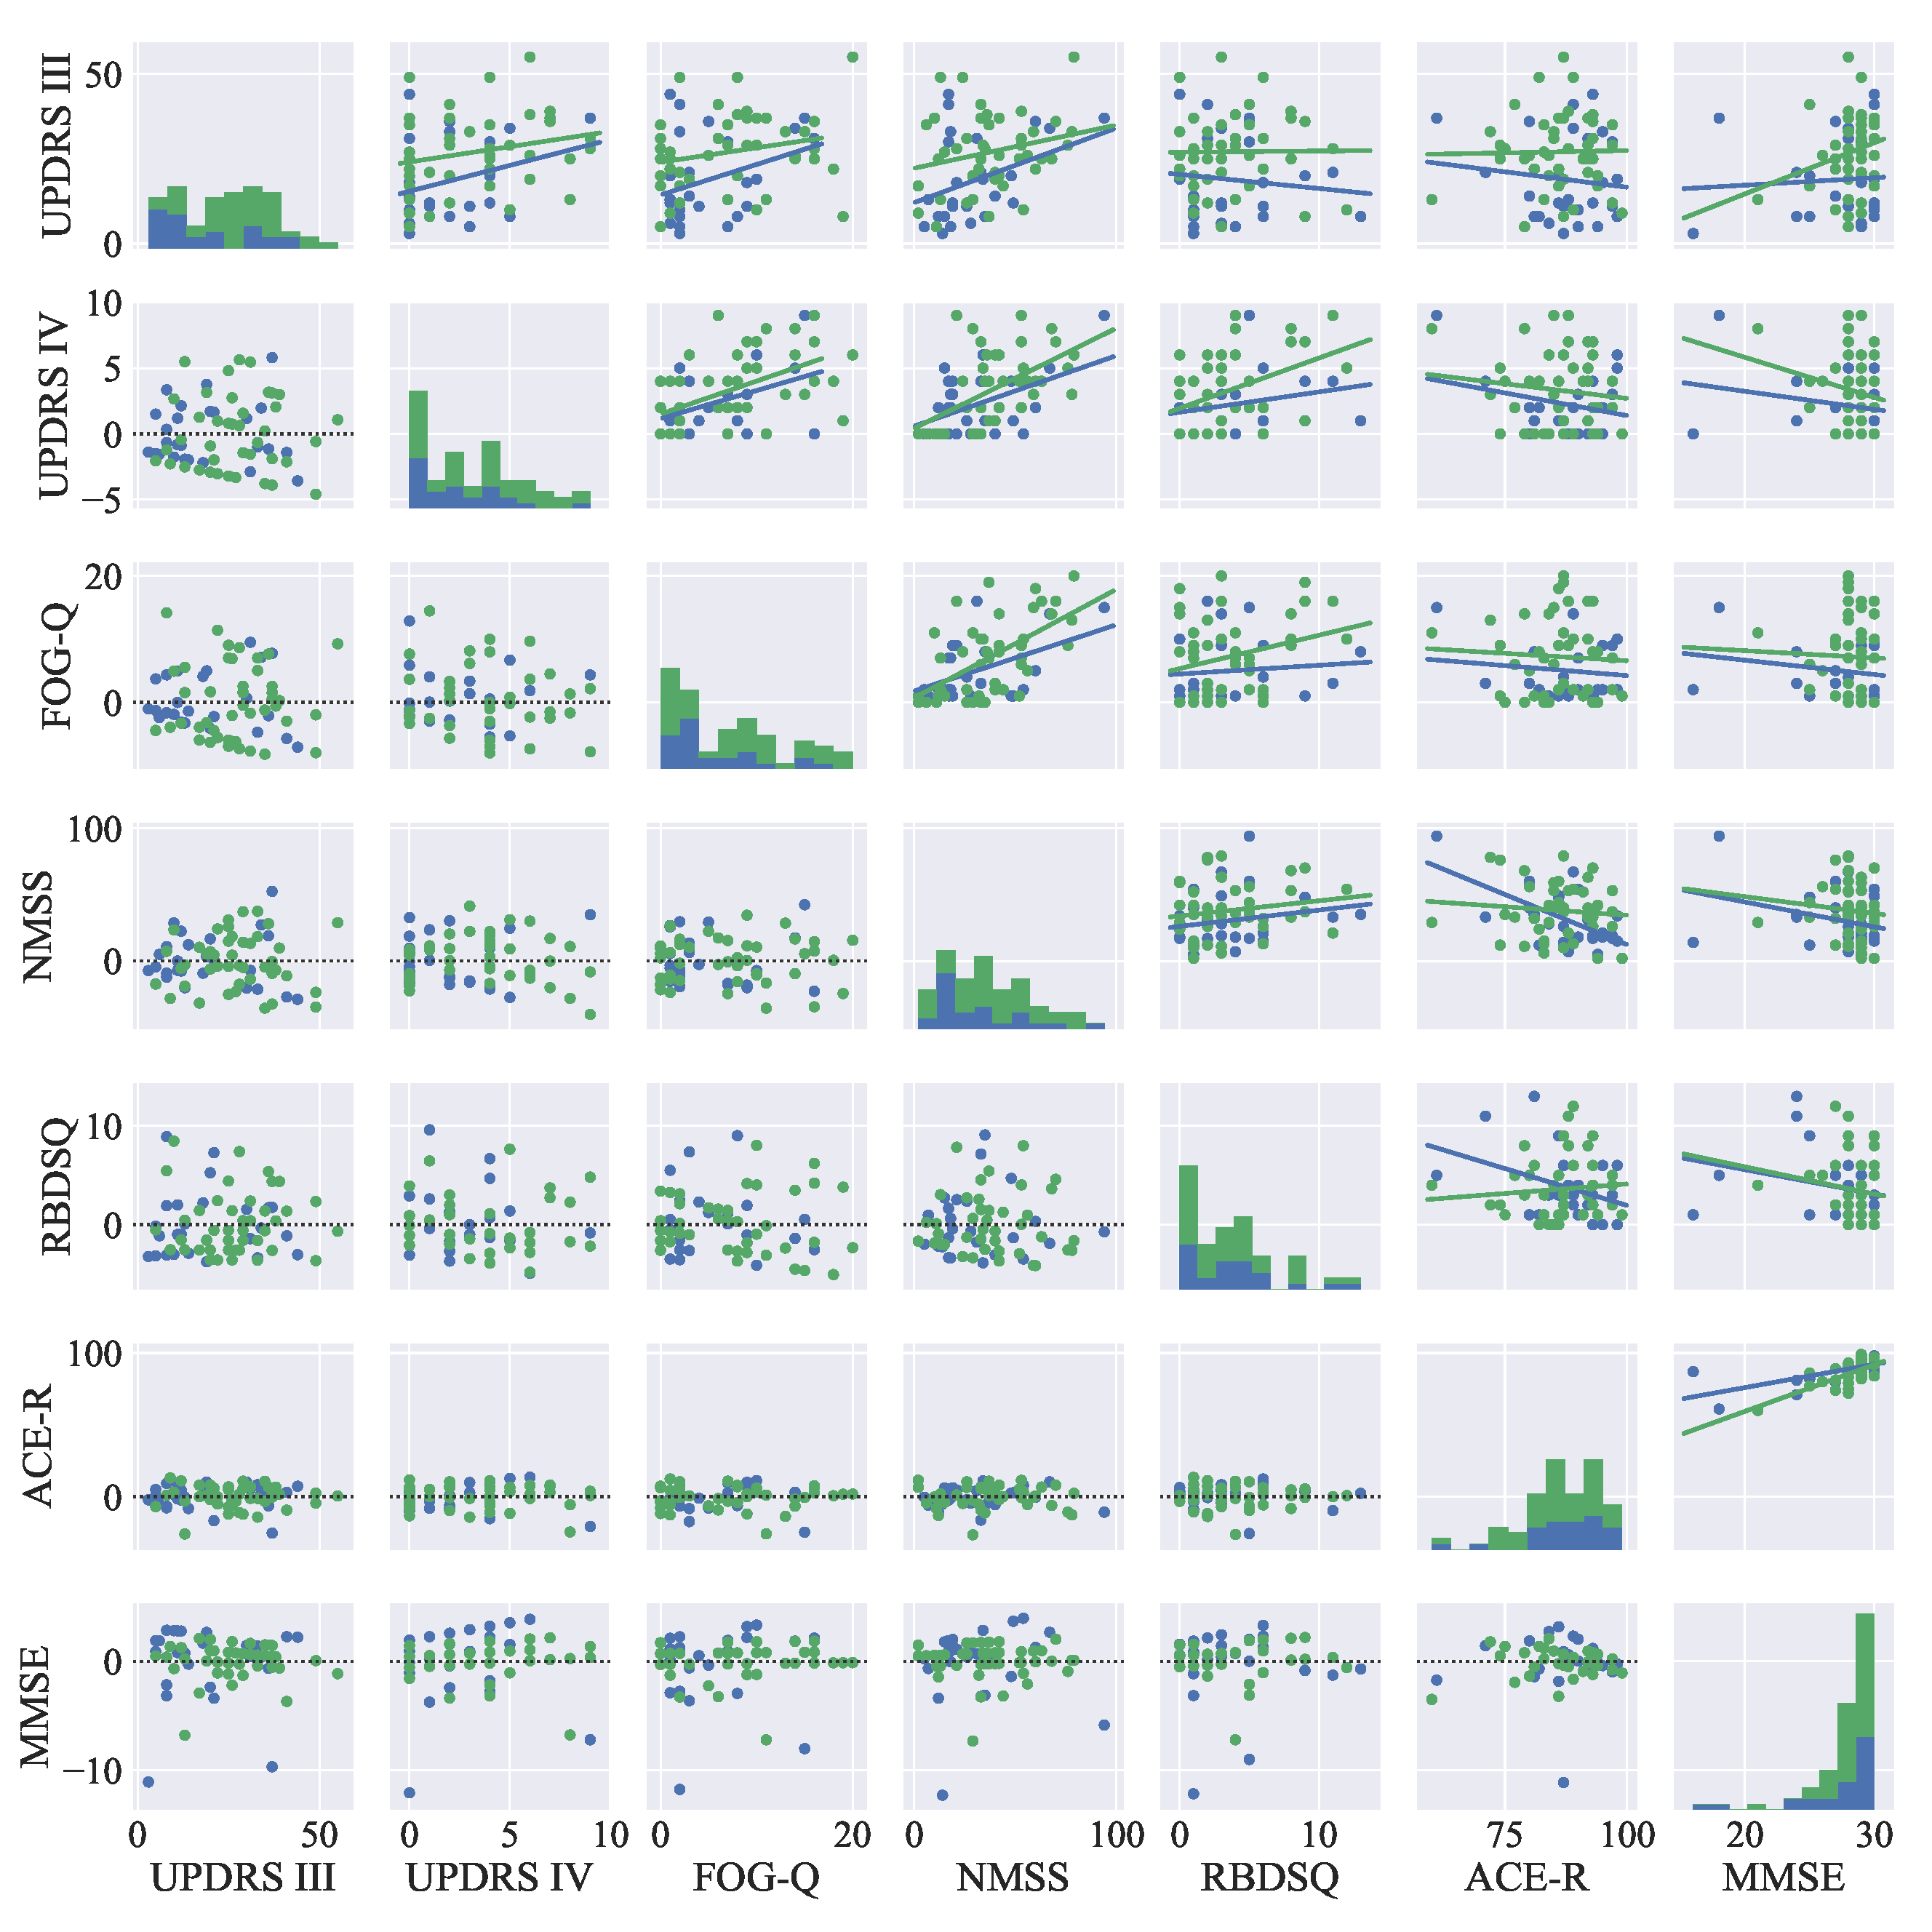
\includegraphics[width=0.99\textwidth]{pictures/ch5_clinical_statistics.eps}
	\caption[Descriptive statistical graphs of clinical data for PD patients.]{Descriptive statistical graphs of clinical characteristics of PD patients participated in this study: on the main diagonal, histograms are visualized. Next, the upper triangular part of the graph-grid shows scatter plots with the fitted lines of the linear regression models. And finally, the lower triangular part of the graph-grid is used to display residuals for the models shown in the the upper grid. Colour notation: blue colour represents female speakers, and green colour represents male speakers. For the description of the rating scales, see Table~\ref{tab:ch5_clinical_data}.}
	\label{fig:ch5_clinical_statistics}
\end{figure}

\subsection{Feature extraction}
\label{ch5_3_2}

As in the case of study presented in Chapter~\ref{ch4}, the following acoustic features quantifying dysprosody in HD were used~\cite{Brabenec2017}. To describe variation in pitch, fundamental frequency (F0) was used, specifically: standard deviation of F0 (FOSD), relative standard deviation of F0 (relF0SD), variation range of F0 (FOVR), and relative variation range of F0 (relF0VR) were computed. Regarding description of variation in intensity, squared energy operator (SEO) and Teager-Kaiser energy operator (TEO) were used, specifically: standard deviation of SEO/TEO (SEOSD/TEOSD), relative standard deviation of SEO/TEO (relSEOSD/relTEOSD), variation range of SEO/TEO (SEOVR/TEOVR), and relative variation range of SEO/TEO (relSEOVR/relTEOVR) were computed. And finally, total speech time (TST), net speech time (NST), total pause time (TPT), total speech rate (TSR), net speech rate (NSR), total pause time (pauses longer than $50$\,ms) (TPT\,($50$\,ms)), articulation rate (AR), and speech index of rhythmicity (SPIR) were computed to describe speech rate and pausing abnormalities.

\subsection{Analytical setup}
\label{ch5_3_3}

To describe the presence of possible relationship between the values of the computed acoustic features quantifying dysprosody in HD and other motor and non-motor symptoms (assessed by the selected clinical rating scales) in PD, Spearman's correlation coefficient ($\rho$) was used (short description of this method can be found in the previous chapter). The significance level of correlation ($p$) of $0.05$ was selected. Due to the limited number of samples and the exploratory character of the study, the correction for multiple comparisons was not performed. Moreover, due to the large number of clinical rating scales under focus, partial correlations were not computed to control for the effect of covariates, but rather classical correlations were applied to provide a~preliminary insight into association between dysprosody in HD and other non-speech symptoms of PD.

Consequently, multivariate regression models estimating values of the analysed clinical rating scales were built ($10$-fold cross-validation with $20$ repetitions was used for validation). However, as in the case of HD identification (see Chapter~\ref{ch4}), not all acoustic features were used for this purpose. As previously, a~modified version of sequential floating forward selection~\cite{Pohjalainen2014} algorithm was applied to reduce the number of features and create the regression models with low dimensionality, better clinical interpretability, and high performance~\cite{Guyon2006}. With respect to the actual regression algorithm, classification and regression trees (CART) were employed. Classification and regression trees are a~non-parametric supervised machine learning algorithm based on mathematical theory introduced in $1984$ by Breiman, Freidman, Olshen and Stone~\cite{Breiman1984} that are still commonly used in the field of biostatistics due to its robustness to outliers and ability to deal with highly dimensional and highly correlated data~\cite{Hastie2009}. The result of the algorithm are often well-interpretable, which makes this algorithm especially attractive.

To measure the prediction performance of the trained models, several conventional and widely-used regression metrics such as mean absolute error (MAE), and root mean squared error (RMSE) were employed. Moreover, a~novel regression metric named estimation error rate (EER) was computed to express the prediction error in percentage, which is particularly useful for easy and fast interpretation. These metrics are defined as:
\begin{eqnarray}
	\mathrm{MAE}  &=& \frac{1}{n}\sum_{i=1}^{n} \abs{y_{i}-\hat{y_{i}}}, \\
	\mathrm{RMSE} &=& \sqrt{\frac{1}{n}\sum_{i=1}^{n} (y_{i}-\hat{y_{i}})^2}, \\
	\mathrm{EER}  &=& \frac{1}{n \cdot r}\sum_{i=1}^{n} \abs{y_{i}-\hat{y_{i}}} \cdot 100\,[\%], 
\end{eqnarray}
where the above mentioned variables stands for: $n$ is the number of true/predicted values, $y_{i}$ and $\hat{y_{i}}$ represents the true and predicted values of the response variable, respectively, and $r$ denotes the range of values of the given clinical rating scale present in the dataset (this is particularly useful when interpreting the values of EER for the restricted range of values that is a~common situation when dealing with the data from patients with neurodegenerative disorders\footnote{It is important to note that every dataset is different in the participants. For instance, in the case of this study, patients with PD were acquired. These patients however are often in the moderate to severe stage of the disease since an accurate early PD diagnosis is rare or completely missing. Therefore, even though the clinical rating scales used to assess the parkinsonian manifestations are able to quantify very mild or severe disabilities, such data is almost never acquired. Hence, the conversion of some classical prediction metric such as mean absolute error into percentage can not simply be done using the range of the clinical rating scales because the resulting estimation error rates would be overestimating the performance of the trained models. For this reason, it is extremely important to consider the actual range of values present in the dataset.}, see Table~\ref{tab:ch5_clinical_data}). In the frame of this study, these regression metrics can be interpreted as: mean absolute error expresses the average absolute difference between the predicted and true values of the variable under focus, so that with higher mean absolute error, worse predictions are made. Root mean squared error expresses the square root of the average of squared prediction errors, so that with lower root mean squared error, even more inaccurate predictions are made. Furthermore, as opposed to RMSE, MAE has the advantage that it describes the prediction error in the same units as the variables themselves. However, RMSE is also frequently used because it amplifies larger differences and is therefore more sensitive to prediction errors. And finally, estimation error rate expresses the mean absolute error in relation to the range of values of the predicted variable, so that it gives the visual impression of the estimation error of the model given the actual statistical properties of the dataset.

\section{Results}
\label{ch5_4}

Results of the correlation analysis are summarized in Table~\ref{tab:ch5_statistical_analysis}. The table shows top three acoustic features sorted according to their significance level of correlation expressed by Spearman's correlation coefficient. The following results showing the correlation for the specific prosodic areas under focus were achieved\footnote{Only a~single statistically significant feature per prosodic area is presented, therefore it might happen that some features will not appear in the summary. Features with $p>0.05$ are not shown as well as they are considered statistically insignificant. For complete picture, see~\ref{tab:ch5_statistical_analysis}} (* means that $p<0.05$; ** means that $p<0.01$; T1\,--\,poem recitation task; T2\,--\, reading with neutral emotion; and T3\,--\,stress-modified reading):
\begin{enumerate}
	\item UPDRS~III\,--\,the strongest correlation was found in the case of features describing reduced variation in pitch and intensity of speech in all three speech tasks (T1--T3) (T1: $-0.38^{**}$ (F0VR), $-0.30^{**}$ (TEOSD); T2: $-0.28^{*}$ (F0SD), $0.28^{*}$ (SEOSD); and T3: $-0.37^{**}$ (F0VR), $-0.30^{*}$ (TEOVR)).
	\item UPDRS~IV\,--\,the strongest correlation was found in the case of features describing reduced variation in intonation (T1, T2), intensity of speech (T3), and speech rate abnormalities (T1, T2) (T1: $0.29^{*}$ (relF0SD), $0.21^{*}$ (TPT\,(50\,ms)); T2: $0.32^{**}$ (relF0SD), $0.31^{**}$ (TPT\,(50\,ms)); and T3: $-0.21^{*}$ (TEOSD), $-0.21^{*}$ (F0VR)).
	\item FOG-Q\,--\,the strongest correlation was found mostly in the case of features describing speech rate abnormalities in all three speech tasks (T1--T3), and reduced variation in intensity of speech (T1) (T1: $-0.35^{**}$ (NST), $0.28^{*}$ (relF0SD); T2: $0.42^{**}$ (TPT\,(50\,ms)); and T3: $-0.27^{*}$ (NST)).
	\item NMSS\,--\,the strongest correlation was found in the case of features describing reduced variation in intonation and intensity of speech in all three speech tasks (T1--T3) (T1: $-0.29^{*}$ (TEOSD), $0.26^{*}$ (relF0SD); T2: $0.36^{*}$ (relF0SD), $0.31^{*}$ (relTEOVR); and T3: $-0.36^{*}$ (TEOVR), $-0.29^{*}$ (F0VR)).
	\item RBDSQ\,--\,the strongest correlation was found only in the case of features describing reduced variation in intensity of speech (T1, T2) (T1: $0.20^{*}$ (TEOSD); and T2: $-0.23^{*}$ (SEOSD)).
	\item ACE-R\,--\,the strongest correlation was found in the case of features describing speech rate abnormalities (T1), and reduced variation in intensity of speech (T3) (T1: $-0.43^{*}$ (TPT); T3: $0.23^{*}$ (TEOSD)).
	\item MMSE\,--\,the strongest correlation was found in the case of a~single feature describing speech rate abnormalities (T1: $-0.26^{*}$ (TPT)).
	\item BDI\,--\,none of the features showed statistically significant correlation.
\end{enumerate}

\begin{table*}[htb!]
	\centering
	\begin{threeparttable}
		\caption{Correlation analysis of the prosodic features.}
		\label{tab:ch5_statistical_analysis}
		\footnotesize
		\centering
		\begin{tabular}{l l r c l r c l r c}

			\hline\hline\noalign{\smallskip}
			\rowcolor{gray_table}
			& \multicolumn{3}{c}{T1} & \multicolumn{3}{c}{T2} & \multicolumn{3}{c}{T3} \\
			\noalign{\smallskip}
			scale & features & $\rho$ & $p$ & features & $\rho$ & $p$ & features & $\rho$ & $p$ \\
			\noalign{\smallskip}\hline\noalign{\smallskip}
			
			\multirow{3}{*}{UPDRS~III} 
			& F0VR  & -0.38 & ** & F0SD  & -0.28 & *  & F0VR  & -0.37 & ** \\
			& TEOSD & -0.30 & ** & SEOSD &  0.28 & *  & F0SD  & -0.34 & ** \\
			& TEOVR & -0.25 & *  & SEOVR &  0.28 & *  & TEOVR & -0.30 & *  \\
			
			\noalign{\smallskip}
			\multirow{3}{*}{UPDRS~IV} 
			& relF0SD       &  0.29 & *  & relF0SD       &  0.32 & ** & TEOSD & -0.21 & *  \\
			& TPT\,(50\,ms) &  0.21 & *  & TPT\,(50\,ms) &  0.31 & ** & F0VR  & -0.21 & *  \\
			& relF0VR       &  0.20 &    & AR            & -0.31 & ** & TEOVR & -0.18 &    \\
			
			\noalign{\smallskip}
			\multirow{3}{*}{FOG-Q} 
			& NST     & -0.35 & ** & TPT\,(50\,ms) &  0.42 & ** & NST & -0.27 & *  \\
			& NSR     &  0.35 & ** & AR            & -0.42 & ** & NSR &  0.27 & *  \\
			& relF0SD &  0.28 & *  & NST           & -0.41 & ** & TST & -0.26 & *  \\
			
			\noalign{\smallskip}
			\multirow{3}{*}{NMSS} 
			& TEOSD   & -0.29 & *  & relF0SD  &  0.36 & ** & TEOVR & -0.36 & ** \\
			& relF0SD &  0.26 & *  & relTEOVR &  0.31 & ** & TEOSD & -0.35 & ** \\
			& TPT     &  0.20 &    & relF0VR  &  0.26 & *  & F0VR  & -0.29 & *  \\
			
			\noalign{\smallskip}
			\multirow{3}{*}{RBDSQ} 
			& TEOSD &  0.20 & *  & SEOSD    & -0.23 & *  & SPIR    & -0.18 &    \\
			& TEOVR &  0.20 &    & relSEOVR &  0.10 &    & TEOSD   &  0.17 &    \\
			& SEOSD & -0.17 &    & SEOVR    & -0.09 &    & relF0SD &  0.17 &    \\
			
			\noalign{\smallskip}
			\multirow{3}{*}{ACE-R} 
			& TPT & -0.43 & ** & TEOSD    &  0.18 &    & TEOSD &  0.23 & *  \\
			& TST & -0.33 & ** & relSEOVR &  0.16 &    & TEOVR &  0.20 &    \\
			& TSR &  0.33 & ** & relF0VR  & -0.16 &    & SPIR  &  0.20 &    \\
			
			\noalign{\smallskip}
			\multirow{3}{*}{MMSE} 
			& TPT      & -0.26 & *  & relTEOVR & -0.17 &    & F0SD          & -0.18 &    \\
			& relSEOSD & -0.17 &    & NST      &  0.16 &    & SEOVR         & -0.13 &    \\
			& TST      & -0.16 &    & TPT      & -0.16 &    & TPT\,(50\,ms) & -0.12 &    \\
			
			\noalign{\smallskip}
			\multirow{3}{*}{BDI} 
			& relTEOVR &  0.18 &    & SEOSD    &  0.21 &    & relTEOSD &  0.18 &    \\
			& SEOSD    &  0.16 &    & relTEOVR &  0.15 &    & relSEOSD & -0.18 &    \\
			& relTEOSD &  0.15 &    & relSEOVR & -0.14 &    & relSEOVR & -0.16 &    \\
			
			\noalign{\smallskip}\hline\hline
		\end{tabular}
		
		\begin{tablenotes}
			\scriptsize
			\item[1] Table notation: T1\,--\,poem recitation task; T2\,--\,emotionally-neutral reading task; T3\,--\,stress-modified reading task; $\rho$~--~Spearman's correlation coefficient; $p$~--~significance level of correlation (* means $p<0.05$; ** means $p<0.01$); UPDRS~III\,--\,Unified Parkinson's disease rating scale, part~III: evaluation of motor function~\cite{Fahn1987}; UPDRS~IV\,--\,Unified Parkinson's disease rating scale, part~IV: evaluation of complications of therapy (Hoehn and Yahr scale, staging of severity of Parkinson's disease)~\cite{Fahn1987}; FOG-Q\,--\,Freezing of gait questionnaire~\cite{Giladi2000}; NMSS\,--\,Non-motor symptoms scale~\cite{Chaudhuri2007}; RBDSQ\,--\,The REM sleep behavior disorder screening questionnaire~\cite{Stiasny2007}; ACE-R\,--\,Addenbrooke's cognitive examination-revised~\cite{Larner2007}; MMSE\,--\,Mini-mental state examination~\cite{Folstein1975}; BDI\,--\,Beck depression inventory \cite{Beck2000, Beck1961}.
		\end{tablenotes}	
	\end{threeparttable}
\end{table*}

Moreover, three specific clinical rating scales were selected: UPDRS~III (evaluation of motor deficits), FOG-Q (evaluation of gait freezing), ACE-R (evaluation of cognitive deficits). For these three scales, regression plots can be seen in Figure~\ref{fig:ch5_correlation_plots}. The figure provides a~visual impression about the strength of a~linear relationship between the most correlated acoustic features and the values of the selected clinical rating scales (a~single feature is chosen for each scenario). 

\begin{figure}[htb!]
	\centering
	\scriptsize
	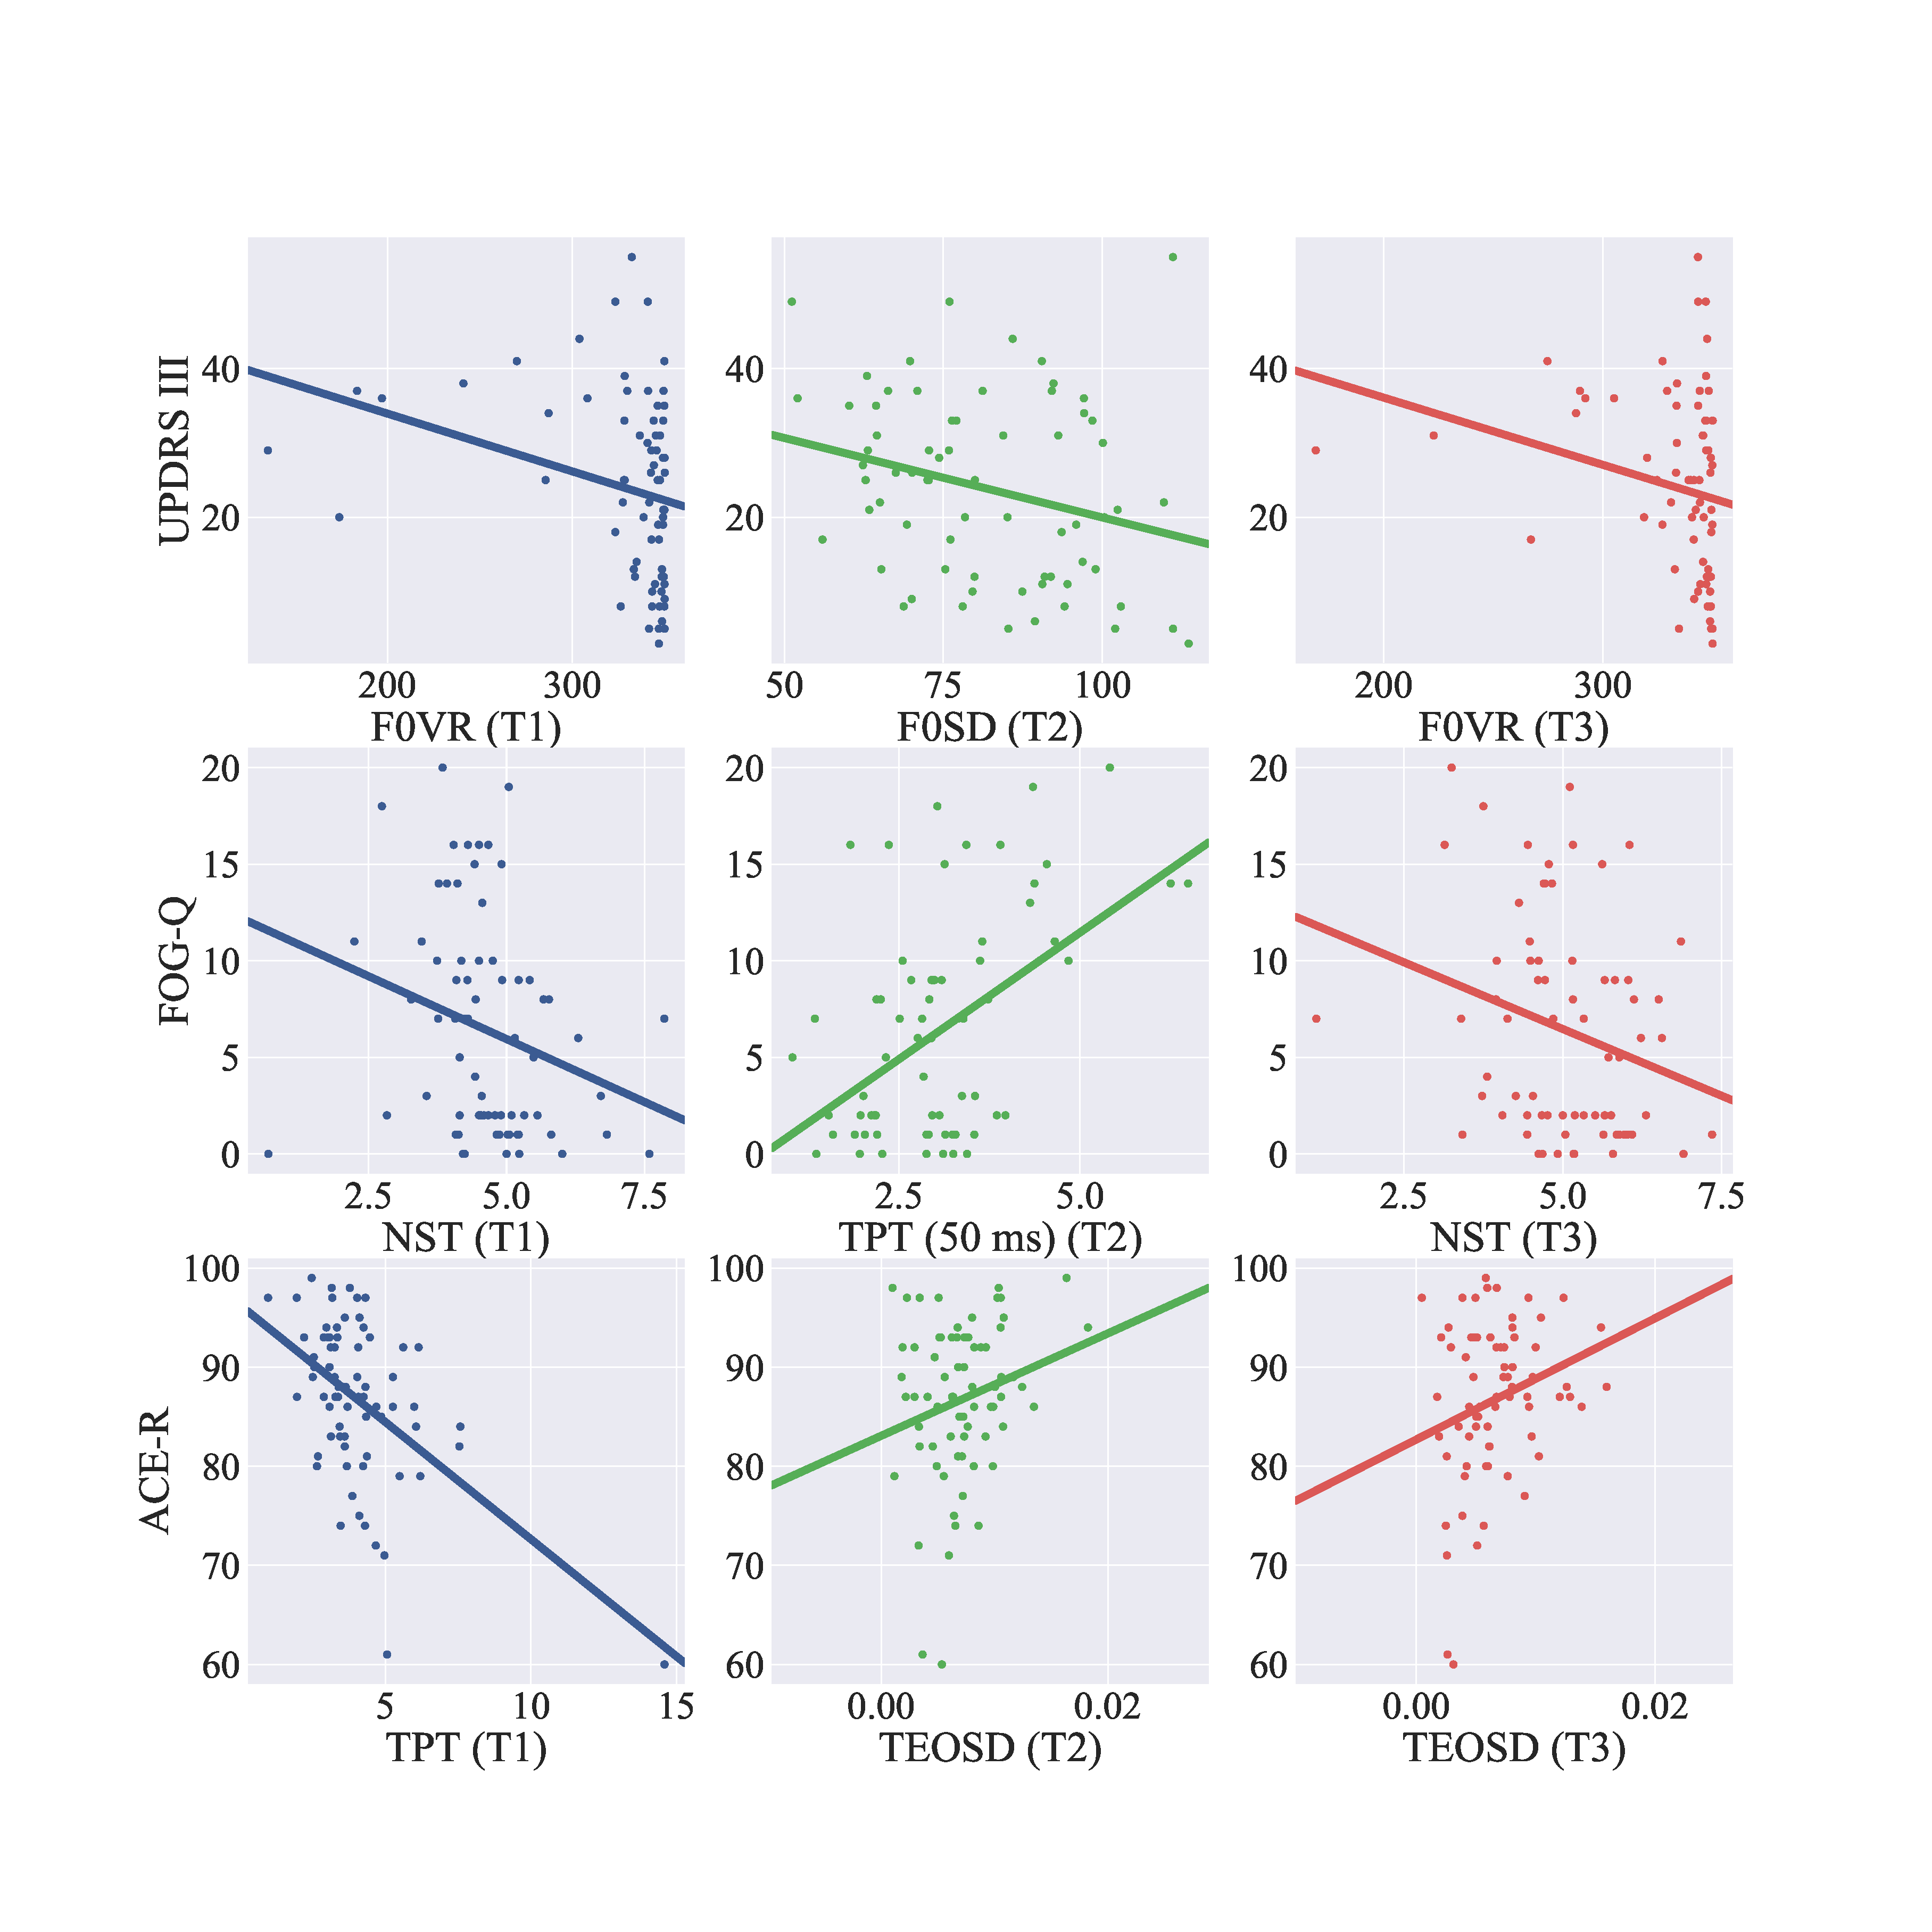
\includegraphics[width=0.99\textwidth]{pictures/ch5_correlation_plots.eps}
	\caption[Regression plots for UPDRS~III, FOG-Q, and ACE-R.]{Regression plots (scatter plots with the fitted line of the robust linear regression estimator) of the selected rating scales (UPDRS~III, FOG-Q, ACE-R) for all three speech tasks performed by all PD patients: T1\,--\,poem recitation task (first column/blue colour); T2\,--\,emotionally-neutral reading (second column/green colour); and T3\,--\,stress-modified reading (third column/red colour). Only one feature for each clinical rating scale/speech feature is visualized (selected according to the Spearman's correlation coefficient, see Table~\ref{tab:ch5_statistical_analysis}). For more information about the acoustic features notation, see Section~\ref{ch5_3_2}.}
	\label{fig:ch5_correlation_plots}
\end{figure}

As can be seen, the strong relationship between reduced variation in pitch and UPDRS~III (in the case of all the three speech tasks) is evident. Specifically, the flatter the intonation, the more severe motor disability assessed by UPDRS~III can be observed. Next, the strong relationship between speech rate/pausing abnormalities and FOG-Q (in the case of all the three speech tasks) is present as well. Specifically, the faster the speech during poem recitation, larger number of pauses (longer that $50$\,ms) during emotionally-neutral reading, and faster the speech during stress-modified reading, the more severe gait freezing episodes assessed by UPDRS~III can be observed. And finally, the strong relationship between speech rate/pausing abnormalities and ACE-R in the case of poem recitation can be seen. For the other two tasks, the association is much weaker (less statistically significant as well). Specifically, the faster speech (less time spent on pausing) during poem recitation, and larger deviation of speech intensity during reading (emotionally-neutral, and stress-modified), the more severe cognitive deficits assessed by ACE-R can be observed. These observations emphasize the fact that poem recitation task is a~great candidate to emphasize monopitch in HD, but also some cognitive deficits that are probably related to worse control of speech tempo (patients try to compensate it by occasional rushes of speech, etc.).

Next, for UPDRS~III, FOG-Q, and ACE-R, multivariate regression models using the features selected by the feature selection algorithm, were built and visualized (visualization of the approximation of decision making performed by the regression tree) using the three graphs, see Figure~\ref{fig:ch5_regression_tree_updrs}, Figure~\ref{fig:ch5_regression_tree_fogq}, and Figure~\ref{fig:ch5_regression_tree_acer}, respectively. Moreover, the results of the multivariate regression analysis are summarized in Table~\ref{tab:ch5_classification_groups}, and Table~\ref{tab:ch5_classification_combination}.

\begin{figure}[htb!]
	\centering
	\scriptsize
	\includegraphics[width=0.99\textwidth]{pictures/ch5_tree_model_updrs.pdf}
	\caption[Regression tree graph visualization for UPDRS~III]{Visualization of the regression tree built to estimate UPDRS~III. The tree was trained using a~single training run applied on all data in the dataset/selected features (hence the decision making of the tree is an approximation of the behavior responsible for the results summarized in Table~\ref{tab:ch5_classification_combination}). In the case of this tree: TST (T2), F0VR (T1), and TEOSD (T1) were used. For explanation of the speech task and acoustic feature notation, see Section~\ref{ch5_3_1}, and Section~\ref{ch5_3_2}, respectively.}
	\label{fig:ch5_regression_tree_updrs}
\end{figure}

\begin{figure}[htb!]
	\centering
	\scriptsize
	\includegraphics[width=0.60\textwidth]{pictures/ch5_tree_model_fogq.pdf}
	\caption[Regression tree graph visualization for FOG-Q]{Visualization of the regression tree built to estimate FOG-Q. The tree was trained using a~single training run applied on all data in the dataset/selected features (hence the decision making of the tree is an approximation of the behavior responsible for the results summarized in Table~\ref{tab:ch5_classification_combination}). In the case of this tree: TPT (T2), F0VR (T1), and SEOVR (T1) were used. For explanation of the speech task and acoustic feature notation, see Section~\ref{ch5_3_1}, and Section~\ref{ch5_3_2}, respectively.}
	\label{fig:ch5_regression_tree_fogq}
\end{figure}

\begin{figure}[htb!]
	\centering
	\scriptsize
	\includegraphics[width=0.60\textwidth]{pictures/ch5_tree_model_acer.pdf}
	\caption[Regression tree graph visualization for ACE-R]{Visualization of the regression tree built to estimate ACE-R. The tree was trained using a~single training run applied on all data in the dataset/selected features (hence the decision making of the tree is an approximation of the behavior responsible for the results summarized in Table~\ref{tab:ch5_classification_combination}). In the case of this tree: TPT (T2), and relSEOSD (T1) were used. For explanation of the speech task and acoustic feature notation, see Section~\ref{ch5_3_1}, and Section~\ref{ch5_3_2}, respectively.}
	\label{fig:ch5_regression_tree_acer}
\end{figure}

\begin{table*}[htb!]
	\centering
	\begin{threeparttable}
		\caption{Results of the regression analysis for individual speech tasks.}
		\label{tab:ch5_classification_groups}
		\footnotesize
		\centering
		\begin{tabular}{l c c c c l}
		
			\hline\hline\noalign{\smallskip}
			\rowcolor{gray_table}
			scale & MAE & RMSE & EER & No. & selected features \\
			\noalign{\smallskip}
			\multicolumn{6}{c}{Poem recitation task} \\
			\noalign{\smallskip}\hline\noalign{\smallskip}
			
			UPDRS III &  9.41~$\pm$~2.73 & 11.45~$\pm$~3.13 & 18.11~$\pm$~5.26 & 2 & F0VR, TEOSD \\
			UPDRS IV  &  2.12~$\pm$~0.65 &  2.69~$\pm$~0.72 & 23.65~$\pm$~7.26 & 1 & relTEOVR \\
			FOG-Q     &  4.52~$\pm$~1.57 &  5.83~$\pm$~1.92 & 22.61~$\pm$~7.89 & 3 & TEOVR, F0VR, TST \\
			NMSS      & 18.55~$\pm$~4.48 & 21.88~$\pm$~4.83 & 20.16~$\pm$~4.87 & 1 & relTEOVR \\
			RBDSQ     &  2.86~$\pm$~0.80 &  3.50~$\pm$~0.94 & 22.06~$\pm$~6.17 & 1 & relSEOVR \\
			ACE-R     &  6.18~$\pm$~1.84 &  7.67~$\pm$~2.23 & 15.86~$\pm$~4.72 & 1 & relSEOSD \\
			MMSE      &  1.83~$\pm$~0.77 &  2.52~$\pm$~1.26 & 13.13~$\pm$~5.50 & 2 & SEOVR, TPT \\
			BDI       &  5.65~$\pm$~1.52 &  6.68~$\pm$~1.80 & 20.94~$\pm$~5.63 & 2 & TPT, relSEOVR \\
			
			\noalign{\smallskip}\hline\noalign{\smallskip}
			\multicolumn{6}{c}{Reading with neutral emotion} \\
			\noalign{\smallskip}\hline\noalign{\smallskip}
			
			UPDRS III & 10.44~$\pm$~2.46 & 12.12~$\pm$~2.63 & 20.08~$\pm$~4.74 & 1 & TPT \\
			UPDRS IV  &  2.31 $\pm$~0.50 &  2.66~$\pm$~0.55 & 25.76~$\pm$~5.63 & 1 & TPT \\
			FOG-Q     &  3.86~$\pm$~1.22 &  4.80~$\pm$~1.42 & 19.31~$\pm$~6.14 & 3 & relF0VR, TPT, NSR \\
			NMSS      & 14.51~$\pm$~4.29 & 17.78~$\pm$~4.98 & 15.78~$\pm$~4.66 & 3 & TPT, relF0SD, TEOSD \\
			RBDSQ     &  2.51~$\pm$~0.68 &  3.04~$\pm$~0.89 & 19.38~$\pm$~5.24 & 1 & TPT \\
			ACE-R     &  6.80~$\pm$~2.12 &  8.34~$\pm$~2.66 & 17.44~$\pm$~5.45 & 1 & TPT \\
			MMSE      &  1.61~$\pm$~0.68 &  2.25~$\pm$~1.24 & 11.50~$\pm$~4.87 & 1 & TPT \\
			BDI       &  4.92~$\pm$~1.39 &  6.00~$\pm$~1.66 & 18.22~$\pm$~5.18 & 1 & TPT \\
			
			\noalign{\smallskip}\hline\noalign{\smallskip}
			\multicolumn{6}{c}{Stress-modified reading} \\
			\noalign{\smallskip}\hline\noalign{\smallskip}
			
			UPDRS III & 10.50~$\pm$~3.23 & 13.10~$\pm$~4.01 & 20.20~$\pm$~6.22 & 2 & relTEOSD, F0SD \\
			UPDRS IV  &  2.45~$\pm$~0.64 &  2.99~$\pm$~0.67 & 27.27~$\pm$~7.16 & 4 & SEOVR, F0VR, AR, TPT \\
			FOG-Q     &  4.90~$\pm$~1.29 &  5.78~$\pm$~1.44 & 24.50~$\pm$~6.47 & 2 & TSR, TST \\
			NMSS      & 17.29~$\pm$~4.88 & 20.91~$\pm$~5.67 & 18.80~$\pm$~5.31 & 1 & TEOVR \\
			RBDSQ     &  2.64~$\pm$~0.71 &  3.23~$\pm$~0.80 & 20.33~$\pm$~5.49 & 2 & TEOSD, F0VR \\
			ACE-R     &  6.18~$\pm$~1.84 &  7.67~$\pm$~2.23 & 15.86~$\pm$~4.72 & 3 & TST, TSR, relSEOSD \\
			MMSE      &  1.76~$\pm$~0.67 &  2.36~$\pm$~1.12 & 12.62~$\pm$~4.83 & 1 & TST \\
			BDI       &  5.44~$\pm$~1.63 &  6.72~$\pm$~1.81 & 20.15~$\pm$~6.04 & 3 & TEOVR, F0VR, SEOSD \\
			
			\noalign{\smallskip}\hline\hline
		\end{tabular}
		
		\begin{tablenotes}
		\scriptsize
			\item[1] Table notation: MAE\,--\,mean absolute error; RMSE\,--\,root mean squared error; EER\,--\,relative estimation error rate (MAE divided by the range of actual values of clinical rating scale present in the dataset; expressed in $\%$); No.\,--\,number of selected features; UPDRS~III\,--\,Unified Parkinson's disease rating scale, part~III: evaluation of motor function~\cite{Fahn1987}; UPDRS~IV\,--\,Unified Parkinson's disease rating scale, part~IV: evaluation of complications of therapy (Hoehn and Yahr scale, staging of severity of Parkinson's disease)~\cite{Fahn1987}; FOG-Q\,--\,Freezing of gait questionnaire~\cite{Giladi2000}; NMSS\,--\,Non-motor symptoms scale~\cite{Chaudhuri2007}; RBDSQ\,--\,The REM sleep behavior disorder screening questionnaire~\cite{Stiasny2007}; ACE-R\,--\,Addenbrooke's cognitive examination-revised~\cite{Larner2007}; MMSE\,--\,Mini-mental state examination~\cite{Folstein1975}; BDI\,--\,Beck depression inventory \cite{Beck2000, Beck1961}.
		\end{tablenotes}
	\end{threeparttable}
\end{table*}

\begin{table*}[htb!]
	\centering
	\begin{threeparttable}
		\caption{Results of the regression analysis for a~combination of speech tasks.}
		\label{tab:ch5_classification_combination}
		\footnotesize
		\centering
		\begin{tabular}{l c c c c l}
		
			\hline\hline\noalign{\smallskip}
			\rowcolor{gray_table}
			scale & MAE & RMSE & EER & No. & selected features \\
			\noalign{\smallskip}\hline\noalign{\smallskip}
			
			UPDRS III &  9.10~$\pm$~2.93 & 11.27~$\pm$~3.46 & 17.52~$\pm$~5.64 & 3 & TST$^{2}$, F0VR$^{1}$, TEOSD$^{1}$ \\
			UPDRS IV  &  2.31~$\pm$~0.50 &  2.65~$\pm$~0.56 & 25.75~$\pm$~5.64 & 1 & TPT$^{2}$ \\
			FOG-Q     &  3.45~$\pm$~1.28 &  4.54~$\pm$~1.61 & 17.28~$\pm$~6.42 & 3 & TPT$^{2}$, F0VR$^{1}$, SEOVR$^{1}$ \\
			NMSS      & 17.03~$\pm$~4.35 & 20.50~$\pm$~4.86 & 18.52~$\pm$~4.73 & 1 & TPT$^{2}$ \\
			RBDSQ     &  2.26~$\pm$~0.83 &  2.88~$\pm$~1.03 & 17.44~$\pm$~6.40 & 3 & F0SD$^{1}$, SEOSD$^{1}$, TPT$^{2}$ \\
			ACE-R     &  6.20~$\pm$~1.85 &  7.68~$\pm$~2.22 & 15.72~$\pm$~4.75 & 2 & TPT$^{2}$, relSEOSD$^{1}$ \\
			MMSE      &  1.60~$\pm$~0.68 &  2.25~$\pm$~1.24 & 11.49~$\pm$~4.92 & 1 & TPT$^{2}$ \\
			BDI       &  4.91~$\pm$~1.40 &  6.00~$\pm$~1.66 & 18.21~$\pm$~5.21 & 1 & TPT$^{2}$ \\
			
			\noalign{\smallskip}\hline\hline
		\end{tabular}
		
		\begin{tablenotes}
		\scriptsize
			\item[1] Table notation: $^{1}$\,--\,poem recitation task; $^{2}$\,--\,reading with neutral emotion; $^{3}$\,--\,stress-modified reading task; MAE\,--\,mean absolute error; RMSE\,--\,root mean squared error; EER\,--\,relative estimation error rate (mean absolute error divided by the range of actual values of clinical rating scale present in the dataset; expressed in $\%$); No.\,--\,number of selected features; UPDRS~III\,--\,Unified Parkinson's disease rating scale, part~III: evaluation of motor function~\cite{Fahn1987}; UPDRS~IV\,--\,Unified Parkinson's disease rating scale, part~IV: evaluation of complications of therapy (Hoehn and Yahr scale, staging of severity of Parkinson's disease)~\cite{Fahn1987}; FOG-Q\,--\,Freezing of gait questionnaire~\cite{Giladi2000}; NMSS\,--\,Non-motor symptoms scale~\cite{Chaudhuri2007}; RBDSQ\,--\,The REM sleep behavior disorder screening questionnaire~\cite{Stiasny2007}; ACE-R\,--\,Addenbrooke's cognitive examination-revised~\cite{Larner2007}; MMSE\,--\,Mini-mental state examination~\cite{Folstein1975}; BDI\,--\,Beck depression inventory \cite{Beck2000, Beck1961}.
		\end{tablenotes}
	\end{threeparttable}
\end{table*}

With respect to the separate analysis (analysis of the speech tasks separately in direction of evaluating their sufficiency to assess severity of PD by estimating the clinical rating scales that are used to assess motor and non-motor deficits occurring with this disease), the following results were achieved: a) T1\,--\,most of the selected acoustic features are based on the description of reduced variability in intonation and intensity of speech. The lowest estimation error rate was obtained in the case of MMSE (SEOVR, TPT): $\mbox{EER}=13.13~\pm~5.50\,\%$, closely followed by ACE-R (relSEOSD): $\mbox{EER}=15.86~\pm~4.72$, and UPDRS~III (F0VR, TEOSD): $\mbox{EER}=18.11~\pm~5.26\,\%$; b) T2\,--\,in $6$ out of the total number of $8$ analysed clinical rating scales, the feature selection found only a~single feature based on the description of speech rate and pausing abnormalities (TPT) to be sufficient enough to describe the relationship between dysprosody in HD and severity of PD. The lowest estimation error rate was obtained in the case of MMSE (TPT): $\mbox{EER}=11.50~\pm~4.87\,\%$; and c) T3\,--\,features based on the description of reduced variability of intensity of speech and speech rate abnormalities dominated most of the models. The lowest estimation error rate was obtained in the case of MMSE (TST): $\mbox{EER}=12.62~\pm~4.83\,\%$, closely followed by ACE-R (TST, TSR, relSEOSD): $\mbox{EER}=15.86~\pm~4.72\,\%$, and NMSS (TEOVR): $\mbox{EER}=18.80~\pm~5.31\,\%$.

Regarding the combined analysis (analysis of the combination of the speech tasks in direction of evaluating the power of the combined model to robustly and complexly assess severity of PD), combination of the speech tasks resulted into lower estimation error rates in most of the cases in which more than a~single acoustic feature was selected. The prediction power of the regression models was slightly improved in the following clinical rating scales (improvements are expressed in \%): $\mbox{UPDRS~III}=0.59\,\%$, $\mbox{FOG-Q}=2.04\,\%$, $\mbox{RBDSQ}=1.94\,\%$. However, as can be seen, in most of the cases, a~single prosodic feature seems to be sufficiently describing a~relationship between dysprosody in HD and other non-speech symptoms occurring with PD. Hypothetically, the prediction power of these models could be increased when taking other HD manifestations into account. Nevertheless, the results clearly show dysprosody is related with other motor (as assessed by UPDRS~III, or FOG-Q) and non-motor (as assessed by MMSE or ACE-R) symptoms in PD.

\section{Conclusion}
\label{ch5_5}

Up to this day, several world-renown researchers analysed relationship between speech disorders in HD and other non-speech symptoms of PD \cite{Goberman2005b, Moreau2007, Skodda2009, Skodda2011c, Skodda2013}. However, investigation of the association between acoustic features quantifying dysprosody in HD and a~complex set of clinical rating scales assessing motor and non-motor symptoms of PD is still rare or missing. This study therefore provides further analysis of the relationship between HD and other aspects of PD using the correlation analysis. Regarding the results, the following conclusion can be made.

Concerning UPDRS~III~\cite{Fahn1987}, the strongest correlation can be observed for the acoustic features describing reduced variation in intonation and intensity of speech. Specifically, in the case of poem recitation task, reduced variation in fundamental frequency was found correlated with higher severity of motor symptoms (F0VR: $-0.38$, $p<0.01$) present in PD, which highlights and confirms the previous findings proposed in Chapter~\ref{ch4} reporting that when PD patients are exposed to additional rhythmical demands, the prosodic deficits occurring with HD gets emphasized. This phenomenon can also be found in the case of stress-modified reading (F0VR: $-0.37$, $p<0.01$) confirming the relevancy of this speech task as well. On top of that, smaller variation and standard deviation of speech intensity was also found correlated with the higher severity of PD for both emotionally-neutral reading (TEOSD: $-0.30$, $p<0.01$) and stress-modified reading (TEOVR: $-0.30$, $p<0.05$). Regarding UPDRS~IV~\cite{Fahn1987}, the strongest correlation can be observed for the acoustic features describing reduced variation in intonation, and speech rate/pausing abnormalities. Interestingly, the best results were achieved for the emotionally-neutral reading task. Specifically, larger standard deviation of fundamental frequency (relF0SD: $0.32$, $p<0.01$), larger number of pauses longer than 50\,ms (TPT\,(50\,ms): $0.31$, $p<0.01$), and slow rate of speech (AR: $-0.31$, $p<0.01$) were found correlated with higher severity of PD. With respect to FOG-Q~\cite{Giladi2000}, the strongest correlation can be observed almost exclusively for the features describing speech rate/pausing abnormalities, which suggests that the relationship between HD and freezing of gait in PD is independent of stress and rhythm. Specifically, larger number of pauses longer than 50\,ms (TPT\,(50\,ms): $0.42$, $p<0.01$), and slow rate of speech (AR: $-0.42$, $p<0.01$) were found correlated with the higher severity of gait freezing in PD. Additionally, statistically significant correlations are present for poem recitation (NST: $-0.35$, $p<0.01$) and stress-modified reading (NST: $-0.27$, $p<0.05$) as well. These results confirm the relationship between the freezing of gait and speech rate disturbances in HD reported by Park et al.~\cite{Park2014} in $2014$. Regarding NMSS~\cite{Chaudhuri2007}, the strongest correlation can be observed for the acoustic features describing reduced variation in intonation and intensity of speech. These acoustic features dominated in the case of all the three speech tasks. Specifically, larger standard deviation of fundamental frequency (relTEOVR: $0.36$, $p<0.01$) and variation in speech intensity (relTEOVR: $0.31$, $p<0.01$) during emotionally-neutral reading, and smaller variation (relTEOVR: $-0.36$, $p<0.01$) and standard deviation (relTEOVR: -$0.35$, $p<0.01$) of speech intensity during stress-modified reading were found correlated with higher severity of non-motor symptoms of PD. In the case of ACE-R~\cite{Larner2007}, the strongest correlation can be observed for the features describing speech rate/pausing abnormalities. Specifically, shorter pauses (TPT: $-0.43$, $p<0.01$) and faster speech (TST: $-0.33$, $p<0.01$) during recitation was found correlated with the cognitive decline in PD. This might mean that PD patients with more severe cognitive manifestations were not able to pay enough attention to precise speech rate, pausing, and timing required by the poem recitation task, so to compensate that, they spoke faster and did not emphasize the end of each verse. These results to some extent confirm the previous finding of Rektorova et al.~\cite{Rektorova2016} reporting that impaired speech rhythmicity predicts rapid cognitive decline in patients with PD. The results for other rating scales are not so convincing, however a~short discussion is provided. Although Rusz et al.~\cite{Rusz2016} revealed that speech impairment is present in approximately $88\,\%$ of patients with idiopathic rapid eye movement sleep behaviour disorder (RBD), only mildly strong connection between reduced variation in speech intensity in HD and sleep disorders in PD assessed by RBDSQ~\cite{Stiasny2007} was found. Next, with respect to MMSE~\cite{Folstein1975}, only a~single acoustic feature describing total duration of speech (TPT: $-0.26$, $p<0.05$) was found correlated with cognitive deficits in PD assessed by this particular rating scale. Finally, despite the fact that some relationship between emotional prosody and depression in PD has already been reported~\cite{Velez2008}, the results of this study did not confirm any particular relationship between prosodic features and depression assessed by BDI~\cite{Beck2000}.

Nowadays, there are some studies focused on the estimation of clinical rating scales assessing severity of PD using the acoustic analysis of dysarthric speech \cite{Asgari2010, Bayestehtashk2015, Eskidere2012, Peterek2013, Tsanas2010, Tsanas2010a, Tsanas2010b, Smekal2015c, Rektorova2016}. However, as mentioned previously, these works mainly estimated UPDRS. Moreover, most of the works only quantified phonatory aspects of HD. This study therefore provides further analysis of computerized remote estimation of motor and non-motor symptoms of PD using the quantification of HD. Regarding the regression analysis, the following conclusions can be drawn.

With respect to the estimation of motor symptoms, it can be concluded that the most interesting results were found in the case of UPDRS~III and FOG-Q. Concerning UPDRS~III~\cite{Fahn1987}, the lowest estimation error ($17.52\,\%$) was achieved for the combined prosodic model composed of three features: TST (emotionally-neutral reading), F0VR (poem recitation task), and TEOSD (stress-modified reading). This shows that every aspect of dysprosody in HD is relevant and useful for estimation of motor symptoms of PD assessed by this particular rating scale. Moreover, it can be seen that these results are consistent with the findings of the correlation analysis showing that speech rate/pausing abnormalities are mostly manifested during reading with neutral emotion, reduced variation in intonation is mostly manifested during poem recitation, and reduced variation in speech intensity is mostly manifested during stress-modified reading. Regarding FOG-Q~\cite{Giladi2000}, the lowest estimation error ($17.28\,\%$) was achieved for the combined prosodic model composed of three features: TPT (emotionally-neutral reading), F0VR (poem recitation task), and SEOVR (stress-modified reading). This also confirms great importance of the robust description of dysprosody when estimating motor deficits in PD. Regarding the estimation of non-motor symptoms, it can be concluded that the most interesting results were found in the case of RBDSQ, ACE-R and MMSE. Concerning RBDSQ~\cite{Stiasny2007}, the lowest estimation error ($17.44\,\%$) was achieved for the combined prosodic model composed of three features: F0SD (poem recitation task), SEOSD (stress-modified reading), and TPT (emotionally-neutral reading). It is therefore evident that when estimating non-motor symptoms of PD, full description of dysprosody is necessary as well. Similarly to the motor aspects, poem recitation task is the preferred choice when quantifying flat speech melody, and speech rate/pausing abnormalities seem to be sufficiently described by emotionally-neutral reading. With respect to ACE-R~\cite{Larner2007}, the lowest estimation error ($15.72\,\%$) was achieved for the combined prosodic model composed of two features: TPT (emotionally-neutral reading), and relSEOSD (poem recitation task). And finally, in the case of MMSE~\cite{Folstein1975}, the lowest estimation error ($15.72\,\%$) was achieved for a~single prosodic feature describing total speech time of the emotionally-neutral reading ($11.49\,\%$). This is in fact the lowest estimation error that was achieved.

To provide relevant discussion and conclusion, limitations of this work need to be pointed out as well. One limitation of this study is the range of values of the rating scales covered by the cohort. This limitation is however tightly linked with the difficulty of the data acquisition in the case of patients in early or severe stages of the disease. On one hand, patients that are diagnosed in the early stages of PD are very hard to find, and on the other hand, patients in the severe stages of PD are very hard to examine because of their medical condition. Therefore, one must take into account the fact that the results presented in this study are limited by the statistical properties of the dataset. Another drawback of this study is the fact that the results are based upon speech tasks of relatively limited length. This however is done purposely in order to propose the results that are in line with the methodology and continuously build on top of the findings summarized in Chapter~\ref{ch4}.

To summarize, it is also evident that speech prosody plays a~great role in linking HD and other non-speech deficits in PD. The results also confirm the potential of the acoustic analysis of dysarthric speech to assess PD. At first, they strongly suggest that using a~recitation and stress-modified tasks can emphasize prosodic deficits in HD and therefore can be used for HD identification, and even non-speech symptoms estimation. Secondly, they show importance of speech rate and pausing abnormalities description, especially during emotionally-neutral reading. And finally, they confirm the previous findings of a~few pilot studies concerning estimation of motor and non-motor symptoms of PD~\cite{Smekal2015c, Rektorova2016}.